% =====================================================================
% Problemas nuevos del segundo examen parcial (2025-2), para el capítulo 3
% (Dinámica newtoniana).
%
% Dónde va: al final de la sección «Ejercicios» del capítulo 3, después del
% \end{enumerate} de «Problemas Cuantitativos Propuestos» y antes de
% \chapter{Electromagnetismo}.
%
% Las soluciones están en soluciones_parcial2_apendice.tex, que va al final
% del apéndice. Cada problema enlaza con su solución mediante \pageref.
%
% Requiere: amsmath, siunitx, enumitem, tikz y hyperref (ya cargados en
% main.tex). No usa librerías de TikZ adicionales.
% =====================================================================

\subsubsection{Problemas del segundo examen parcial}
\label{sec:problemas-parcial2}

Los siguientes problemas hicieron parte del segundo examen parcial. Las
soluciones completas están en el apéndice, en la
sección~\ref{sec:soluciones-parcial2}. Intente resolverlos antes de
consultarlas.

\begin{enumerate}[label=\textbf{P\arabic*.}, ref=P\arabic*, leftmargin=*]

    % ----- Energía -----------------------------------------------------
    \item\label{prob:parcial2-caida} \textbf{Caída libre y energía:}
    Se suelta una piedra desde el reposo a una altura $h$ sobre el suelo.
    Desprecie la fricción con el aire.
    \begin{enumerate}
        \item Igualando la energía mecánica arriba y justo antes de tocar el
        suelo, demuestre que la rapidez de llegada es $v = \sqrt{2gh}$.
        \item Calcule $v$ para $h = \SI{20}{\meter}$ y
        $g = \SI{9.8}{\meter\per\second\squared}$.
    \end{enumerate}
    \hfill\textit{[Solución: p.~\pageref{sol:parcial2-caida}]}

    \item\label{prob:parcial2-montana} \textbf{Montaña rusa sin fricción:}
    Un carro de una montaña rusa parte del reposo en el punto $A$, a
    \SI{20}{\meter} de altura, y recorre la vía de la
    figura~\ref{fig:parcial2-montana}. Desprecie toda fricción y tome
    $g = \SI{9.8}{\meter\per\second\squared}$.

    \begin{figure}[htbp]
        \centering
        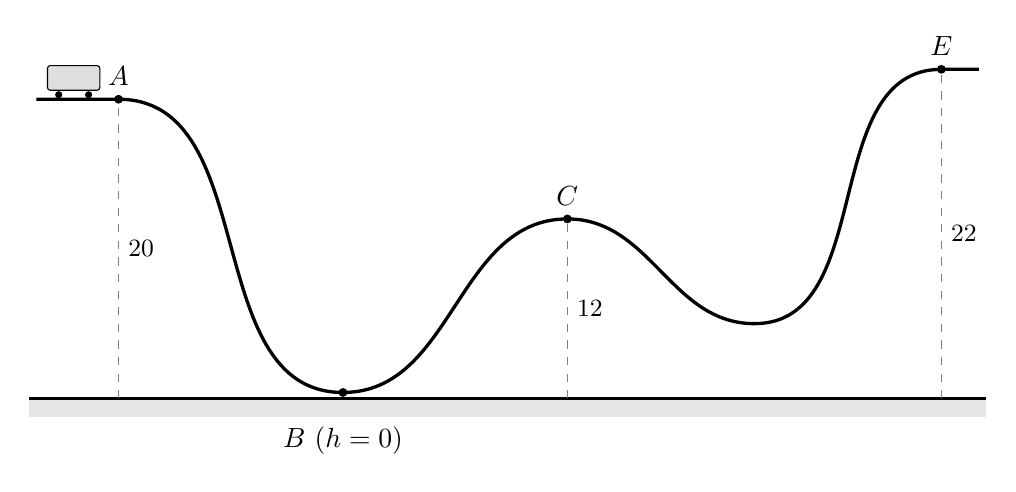
\begin{tikzpicture}[x=0.95cm, y=0.95cm]
            % suelo
            \fill[gray!20] (-1.2,-0.25) rectangle (11.6,0);
            \draw[thick] (-1.2,0) -- (11.6,0);
            % vía
            \draw[very thick] (-1.1,4) -- (0,4) to[out=0,in=180] (3,0.08)
                to[out=0,in=180] (6,2.4) to[out=0,in=180] (8.5,1)
                to[out=0,in=180] (11,4.4) -- (11.5,4.4);
            % alturas
            \foreach \x/\y/\p/\h in {0/4/A/20, 6/2.4/C/12, 11/4.4/E/22} {
                \draw[dashed, gray] (\x,0) -- (\x,\y);
                \fill (\x,\y) circle (1.6pt);
                \node[above] at (\x,\y+0.05) {$\p$};
                \node[right, font=\small] at (\x,\y/2) {\SI{\h}{\meter}};
            }
            \fill (3,0.08) circle (1.6pt);
            \node[below] at (3,-0.25) {$B$ ($h = 0$)};
            % carro en A
            \draw[fill=gray!25, rounded corners=1pt] (-0.95,4.12) rectangle (-0.25,4.45);
            \fill (-0.8,4.06) circle (1.3pt) (-0.4,4.06) circle (1.3pt);
        \end{tikzpicture}
        \caption{Vía de la montaña rusa del problema~\ref{prob:parcial2-montana}.
        El carro parte del reposo en $A$.}
        \label{fig:parcial2-montana}
    \end{figure}

    \begin{enumerate}
        \item Calcule la rapidez del carro en $B$, el punto más bajo, y en la
        cima $C$.
        \item ¿Llega el carro hasta $E$, a \SI{22}{\meter}? ¿Cuál es la altura
        máxima que puede tener una colina para que el carro la supere?
        \item ¿Cambian las respuestas anteriores si el carro va lleno y tiene
        el doble de masa? Explique.
    \end{enumerate}
    \hfill\textit{[Solución: p.~\pageref{sol:parcial2-montana}]}

    \item\label{prob:parcial2-rebote} \textbf{Energía perdida en un rebote:}
    Una pelota de \SI{0.5}{\kilogram} se suelta desde el reposo a
    \SI{10}{\meter} de altura, rebota en el suelo y sube hasta
    \SI{8}{\meter}. Desprecie la fricción con el aire y tome
    $g = \SI{10}{\meter\per\second\squared}$.
    \begin{enumerate}
        \item Calcule la energía mecánica de la pelota al soltarla y en el
        punto más alto después del rebote. ¿Cuánta energía se perdió en el
        rebote y qué porcentaje es de la inicial?
        \item Calcule la rapidez de la pelota justo antes y justo después de
        tocar el suelo.
        \item ¿En qué se transformó la energía perdida?
    \end{enumerate}
    \hfill\textit{[Solución: p.~\pageref{sol:parcial2-rebote}]}

    \item\label{prob:parcial2-lanzamiento} \textbf{Reponer la energía del
    rebote:} Una pelota pequeña de caucho pierde en cada rebote el
    \SI{20}{\percent} de su energía mecánica. Desde una altura
    $h = \SI{10}{\meter}$ se lanza verticalmente con una rapidez $v_0$.
    Desprecie la fricción con el aire y tome
    $g = \SI{9.8}{\meter\per\second\squared}$.
    \begin{enumerate}
        \item ¿Con qué rapidez $v_0$ hay que lanzarla para que, después de
        rebotar, suba exactamente hasta la altura de partida? Demuestre
        primero que $v_0 = \sqrt{gh/2}$.
        \item ¿Importa si se lanza hacia arriba o hacia abajo? Explique.
    \end{enumerate}
    \hfill\textit{[Solución: p.~\pageref{sol:parcial2-lanzamiento}]}

    \item\label{prob:parcial2-frenado} \textbf{Distancia de frenado:} Un
    carro que va con rapidez $v_0$ frena con las llantas bloqueadas sobre una
    carretera horizontal. La fuerza de fricción tiene magnitud
    $f = \mu m g$, donde $\mu$ es el coeficiente de fricción y $m$ la masa
    del carro.
    \begin{enumerate}
        \item Igualando el trabajo de la fuerza de fricción, $W = -f\,d$, con
        el cambio de la energía cinética, demuestre que la distancia de
        frenado es
        \begin{equation*}
            d = \frac{v_0^2}{2\mu g}\,.
        \end{equation*}
        \item ¿La distancia de frenado depende de la masa del carro? Explique
        con base en la expresión anterior.
        \item Calcule $d$ para $v_0 = \SI{20}{\meter\per\second}$
        (\SI{72}{\kilo\meter\per\hour}), $\mu = 0.7$ y
        $g = \SI{9.8}{\meter\per\second\squared}$. ¿Cuántas veces mayor es la
        distancia de frenado si la rapidez se duplica?
    \end{enumerate}
    \hfill\textit{[Solución: p.~\pageref{sol:parcial2-frenado}]}

    % ----- Cantidad de movimiento -------------------------------------
    \item\label{prob:parcial2-impulso} \textbf{Impulso de un bate:} Una
    pelota de béisbol de \SI{0.15}{\kilogram} llega al bate con una rapidez
    de \SI{40}{\meter\per\second} y sale en la dirección contraria con la
    misma rapidez. El contacto dura $\Delta t = \SI{2}{\milli\second}$.
    Calcule la magnitud del cambio en la cantidad de movimiento,
    $\lvert\Delta p\rvert$, y la fuerza media que hace el bate, usando la ley
    de la fuerza $F = \Delta p/\Delta t$.
    \hfill\textit{[Solución: p.~\pageref{sol:parcial2-impulso}]}

    \item\label{prob:parcial2-camion} \textbf{Carro contra camión
    (conceptual):}
    \begin{enumerate}[label=(\Roman*)]
        \item Un carro pequeño choca de frente contra un camión pesado.
        Durante el choque, ¿cuál de los siguientes enunciados es correcto?
        \begin{enumerate}[label=\alph*)]
            \item La fuerza del camión sobre el carro es mayor que la fuerza
            del carro sobre el camión.
            \item La fuerza del carro sobre el camión es mayor que la fuerza
            del camión sobre el carro.
            \item Las dos fuerzas tienen la misma magnitud y direcciones
            opuestas.
            \item Depende de cuál de los dos vehículos iba más rápido.
        \end{enumerate}
        \item ¿Cuál de los dos vehículos sufre el mayor cambio de velocidad?
        Justifique con la ley de la fuerza,
        $\boldsymbol{F} = \Delta\boldsymbol{p}/\Delta t$.
    \end{enumerate}
    \hfill\textit{[Solución: p.~\pageref{sol:parcial2-camion}]}

    \item\label{prob:parcial2-patinadores} \textbf{Dos patinadores se
    empujan:} Dos patinadores, de masas $m_1 = \SI{50}{\kilogram}$ y
    $m_2 = \SI{75}{\kilogram}$, están en reposo sobre el hielo y se empujan.
    Si el primero sale con una velocidad de \SI{3}{\meter\per\second} hacia
    la derecha, use la conservación de la cantidad de movimiento para hallar
    la velocidad del segundo.
    \hfill\textit{[Solución: p.~\pageref{sol:parcial2-patinadores}]}

    \item\label{prob:parcial2-choque} \textbf{Choque en el que los carros
    quedan pegados:} Un carro de masa $m_1$ que se mueve con rapidez $v$
    choca contra un carro de masa $m_2$ que está en reposo, y los dos quedan
    pegados.
    \begin{enumerate}
        \item Escriba la conservación de la cantidad de movimiento antes y
        después del choque y despeje la rapidez final $v_f$ de los dos carros
        juntos.
        \item Demuestre que la energía cinética final es
        \begin{equation*}
            K_f = \frac{m_1}{m_1 + m_2}\,K_i\,,
        \end{equation*}
        donde $K_i = \tfrac{1}{2}m_1 v^2$ es la energía cinética inicial.
        \item Si $m_1 = \SI{1000}{\kilogram}$, $m_2 = \SI{1500}{\kilogram}$ y
        $v = \SI{20}{\meter\per\second}$, calcule $v_f$ y el porcentaje de la
        energía cinética inicial que se pierde en el choque.
    \end{enumerate}
    \hfill\textit{[Solución: p.~\pageref{sol:parcial2-choque}]}

    % ----- Momento angular --------------------------------------------
    \item\label{prob:parcial2-cometa} \textbf{El cometa Halley:} El cometa
    Halley se acerca al Sol hasta una distancia $r_p = \SI{0.59}{UA}$
    (perihelio), donde su rapidez es $v_p = \SI{54}{\kilo\meter\per\second}$,
    y se aleja hasta $r_a = \SI{35}{UA}$ (afelio). En el perihelio y en el
    afelio la velocidad es perpendicular a la posición $\boldsymbol{r}$
    medida desde el Sol, de modo que la magnitud del momento angular es
    $L = m\,r\,v$.
    \begin{enumerate}
        \item ¿Por qué se conserva el momento angular del cometa respecto al
        Sol? (Ayuda: ¿cuánto vale el torque
        $\boldsymbol{\tau} = \boldsymbol{r}\times\boldsymbol{F}$ de una fuerza
        dirigida hacia el Sol?)
        \item Igualando el momento angular en el perihelio y en el afelio,
        despeje la rapidez $v_a$ en el afelio y calcúlela.
    \end{enumerate}
    \hfill\textit{[Solución: p.~\pageref{sol:parcial2-cometa}]}

    \item\label{prob:parcial2-patinadora} \textbf{La patinadora que recoge
    los brazos (conceptual):} Una patinadora gira sobre la punta de un patín
    con los brazos extendidos y luego los recoge contra el cuerpo. El torque
    externo sobre ella es prácticamente cero. ¿Qué pasa con su rapidez de
    giro?
    \begin{enumerate}[label=\alph*)]
        \item Disminuye, porque recoger los brazos cuesta energía.
        \item Aumenta, porque su momento angular se conserva y sus brazos
        quedan a menor distancia $r$ del eje.
        \item No cambia, porque no hay torque externo.
        \item Se detiene, porque desaparece el giro de los brazos.
    \end{enumerate}
    \hfill\textit{[Solución: p.~\pageref{sol:parcial2-patinadora}]}

\end{enumerate}
